\documentclass[tikz,border=2mm]{standalone}
\tikzset{global scale/.style={
    	scale=#1,
    	every node/.append style={scale=#1}
  	}
}
\begin{document}
	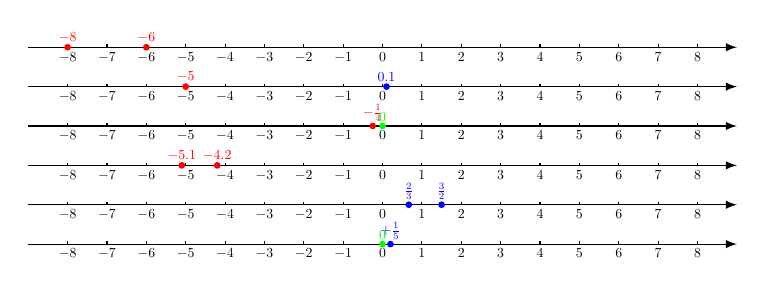
\begin{tikzpicture}[global scale = 0.5]
  		\draw [black, -latex] (-9,0) -- (9,0); 
		\foreach \x in {-8, ..., 8}
			\draw (\x cm,2pt) -- (\x cm,0pt) node[anchor=north] {$\x$};
		% -8, -6, -5, 0.1, -1/4, 0, -4.2, -5.1, 2/3, 3/2, +1/5, 0
		\draw [red, fill=red] (-8, 0) circle(2pt) node [above] {$-8$}; 
		\draw [red, fill=red] (-6, 0) circle(2pt) node [above] {$-6$}; 	
		
		\draw [black, -latex] (-9,-1) -- (9,-1); 
		\foreach \x in {-8, ..., 8}
			\draw (\x cm,-1cm+2pt) -- (\x cm,-1cm+0pt) node[anchor=north] {$\x$};
		% -8, -6, -5, 0.1, -1/4, 0, -4.2, -5.1, 2/3, 3/2, +1/5, 0
		\draw [red, fill=red] (-5, -1) circle(2pt) node [above] {$-5$}; 
		\draw [blue, fill=blue] (0.1, -1) circle(2pt) node [above] {$0.1$}; 			

		\draw [black,  -latex] (-9,-2) -- (9,-2); 
		\foreach \x in {-8, ..., 8}
			\draw (\x cm,-2cm+2pt) -- (\x cm,-2cm+0pt) node[anchor=north] {$\x$};
		% -8, -6, -5, 0.1, -1/4, 0, -4.2, -5.1, 2/3, 3/2, +1/5, 0
		\draw [red, fill=red] (-1/4, -2) circle(2pt) node [above] {$-\frac{1}{4}$}; 
		\draw [green, fill=green] (0, -2) circle(2pt) node [above] {$0$}; 

		\draw [black,  -latex] (-9,-3) -- (9,-3); 
		\foreach \x in {-8, ..., 8}
			\draw (\x cm,-3cm+2pt) -- (\x cm,-3cm+0pt) node[anchor=north] {$\x$};
		% -8, -6, -5, 0.1, -1/4, 0, -4.2, -5.1, 2/3, 3/2, +1/5, 0
		\draw [red, fill=red] (-4.2, -3) circle(2pt) node [above] {$-4.2$}; 
		\draw [red, fill=red] (-5.1, -3) circle(2pt) node [above] {$-5.1$}; 

		\draw [black,  -latex] (-9,-4) -- (9,-4); 
		\foreach \x in {-8, ..., 8}
			\draw (\x cm,-4cm+2pt) -- (\x cm,-4cm+0pt) node[anchor=north] {$\x$};
		% -8, -6, -5, 0.1, -1/4, 0, -4.2, -5.1, 2/3, 3/2, +1/5, 0
		\draw [blue, fill=blue] (2/3, -4) circle(2pt) node [above] {$\frac{2}{3}$}; 
		\draw [blue, fill=blue] (3/2, -4) circle(2pt) node [above] {$\frac{3}{2}$}; 		
			
		\draw [black,  -latex] (-9,-5) -- (9,-5); 
		\foreach \x in {-8, ..., 8}
			\draw (\x cm,-5cm+2pt) -- (\x cm,-5cm+0pt) node[anchor=north] {$\x$};
		% -8, -6, -5, 0.1, -1/4, 0, -4.2, -5.1, 2/3, 3/2, +1/5, 0
		\draw [blue, fill=blue] (1/5, -5) circle(2pt) node [above] {$+\frac{1}{5}$}; 
		\draw [green, fill=green] (0, -5) circle(2pt) node [above] {$0$}; 	
					 			
	\end{tikzpicture}    
\end{document}
